\section[Orientation color detector (Triangle tracker)]{Orientation color detector}
\label{sec:ocd}

\subsection{Introduction}
\label{sec:ocd:intro}

As the first detector was not stable enough, I built a second detector 
that detects dots within a given color range. Three dots are selected 
and it then calculates the angle of the height of the resulting triangle. 
In order to work properly, two points must be clearly closer to form a 
triangle that is near to be isosceles. (figure \ref{fig:ocdorientation})

This detector has been split and renamed by Thomas Lampe. 
To use a similar detector, 
use the ColorDetector and the 
TriangleTracker. See the \ref{sec:ocd:edit} section for more 
information.



\subsection{Detection of the object and his orientation.}
\label{sec:ocd:detection}

    \marginpar{
        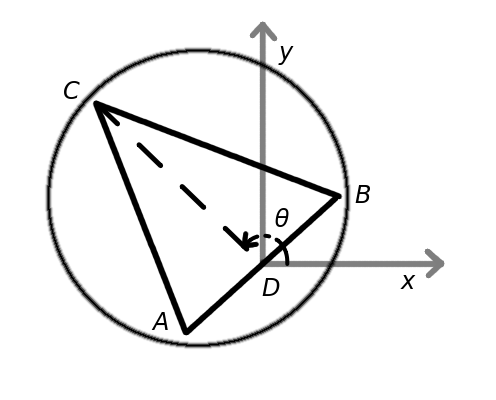
\includegraphics[width=5cm]{./img/orientation.png}
        \captionof{figure}[Calculation of the orientation]{%
        The orientation $\theta$ is the angle between the
        line $\overline{CD}$ and the $x$ axis. It ranges
        counterclockwise from 0 to 2$\pi$.}
        \label{fig:ocdorientation}
    }

\begin{figure}
    \caption{Detection of the position and orientation}
    \begin{subfigure}[h]{0.50\textwidth}
        \centering
        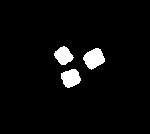
\includegraphics[width=0.80\textwidth]{./img/OrientationDetector_detect.png}
        \caption[Detection of the points]{Detection of the points --
        
        The points are detected and their size are evaluted to 
        discriminate them from noise}
        \label{fig:ocdpointdetection}
    \end{subfigure}
    ~
    \begin{subfigure}[h]{0.50\textwidth}
        \centering
        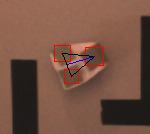
\includegraphics[width=0.80\textwidth]{./img/OrientationDetector_image.png}
        \caption[Detection of the orientation]{Detection of the 
        orientation --

        The points positions are evaluated and the orientation is 
        calculated from point C to D (see figure \ref{fig:ocdorientation})}
        \label{fig:ocdorientationdetection}
    \end{subfigure}
    \label{fig:ocdpodetection}
\end{figure}

The detector enhance the colors given the \_saturation and \_brightness 
values. It then detects blobs using the opencv function cvInRangeS() 
(figure \ref{fig:ocdpointdetection}).
Once the blobs are detected, it selects the three biggest blobs. The 
two closer blobs are used to calculate the line from middle point D to C (figure 
\ref{fig:ocdorientation}). 
The angle theta is the orientation of the object (figure \ref{fig:ocdorientationdetection}).
\\
\\
The position of the object is the mean position of the three points

\subsection{Improvements}
\label{sec:ocd:improvements}

There is less noise than in the previous detector, but it is still 
weak to noise. If one of the dots is not correctly detected and get 
smaller than some noisy blobs, the noisy blob is detected as one of 
the dots and the calculated position is not good.

We could keep the three points in memory and take the closest points 
at the next detection. It could still be unstable if the movement is 
fast and noise is closer than the next position. The best option may 
be to weight the distances with the size of the blobs. 

The drawback compared to Histogram detector is that we need to find 
the best color range at the beginning of every set of experiment, 
because the ambient light may be different from a day to another. When 
this is done, it is a lot more stable than histogram detector but it 
is still vulnerable to changing of ambient light. In overall, the changes 
in the color range at the beginning of a new set of experiment are 
small or inexistent.

The big advantage compared to Histogram detector is that we do not need 
the get the object out of the vision every time we start again the 
detector. 

    \marginpar{
        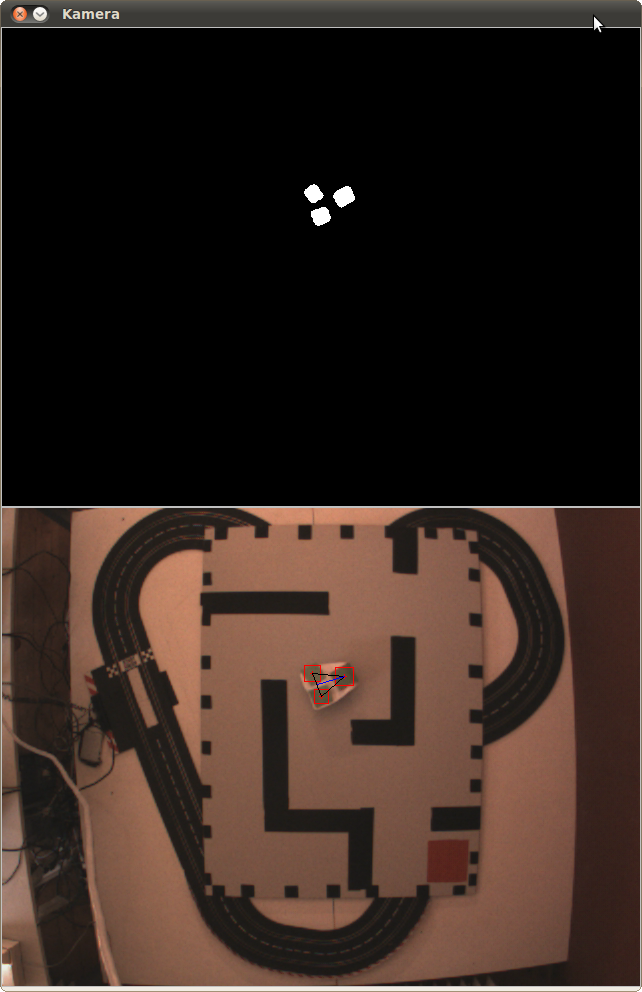
\includegraphics[width=4.5cm]{./img/OrientationDetector_full.png}
        \captionof{figure}[Interface example of the Orientation color
        detector]{Interface example of the Orientation color
        detector -- The detected points (white on black) are above and 
        the calculated 
        triangle and orientation are underneath}
        \label{fig:ocdinterface}
    }

\subsection{How to use}
\label{sec:ocd:howto}
    \begin{enumerate}
        \item Before choosing a color, you may test which one is easier 
        to detect with this detector, given the color in the environment. 
        Square of colored paper seems to fare better than colored 
        dots with pencils on white paper. Take a look at the keys section
        \ref{sec:ocd:howto:keys} to modify the color and range value so
        you can find the best ones for you colored object.
        \item Put 3 dots of the found color on the object you want to 
        detect. Inclined surface reflects less strong light 
            and thus is easier to detect.
        \item Start the detector. The object can be already in the vision 
        or not, it doesn’t matter for this detector. 
        \item Use the keys to change the color range in order to find the 
        best color range for a stable detection. You may have to play
        with it times to times due to different sua nlights. 
        \item Print the color range to the screen, remember it and write 
        it down in the configuration file so you do not have to modify it 
        at each start.
    \end{enumerate}

\subsubsection{Parameters for configuration file}
\label{sec:ocd:howto:params}
    \begin{description} \itemindent=-15pt
        \item[box] \hfill \\ draw box for detected blobs (default true)
        \item[area] \hfill \\ min max minimal and maximal blob sizes
        \item[color] \hfill \\ R G B (mean color)
        \item[wide] \hfill \\ R G B (ranges)
        \item[saturation] \hfill \\ level of saturation (default 0)
        \item[brightness] \hfill \\ level of brightness (default 0)
    \end{description}

\subsubsection{Keys}
\label{sec:ocd:howto:keys}
    \begin{description} \itemindent=-15pt
        \item['4'] R+ 1
        \item['r'] R- 1
        \item['5'] G+ 1
        \item['t'] G- 1
        \item['6'] B+ 1
        \item['y'] B- 1
    \end{description}
    \vspace{5pt}
    \begin{description} \itemindent=-15pt
        \item['7'] Rrange+ 1
        \item['u'] Rrange- 1
        \item['8'] Grange+ 1
        \item['i'] Grange- 1
        \item['9'] Brange+ 1
        \item['o'] Brange- 1
    \end{description}
    \vspace{5pt}
    \begin{description} \itemindent=-15pt
        \item['b'] change brightness mode
        \begin{description}
            \item[upkey] Brightness+ 1
            \item[downkey] Brightness- 1
        \end{description}
    \end{description}
    \vspace{5pt}
    \begin{description} \itemindent=-15pt
        \item['s'] change saturation mode
        \begin{description}
            \item[upkey] Saturation+ 1
            \item[downkey] Saturation- 1
        \end{description}
    \end{description}
    \vspace{5pt}
    \begin{description} \itemindent=-15pt
        \item['p'] Print color/range or brightness or saturation based on 
        current mode
        \item['e'] Get out of brightness/saturation mode (to color/range 
        mode)
    \end{description}
   
\subsection{Edit}
\label{sec:ocd:edit}

During the refactoring of the modules to make them compatible with the 
new Tapir interface, Thomas Lampe have separated the detection and blob 
selection process. He placed the selection process in a TriangleTracker, 
which makes more sense since it is a tracking process. The detector was 
renamed ColorDetector. The major improvements to stabilise more the 
detection of the triangle will now lie in the TriangleTracker rather 
than in the ColorDetector.
